%
% main.tex
%
% Copyright (C) 2021 by SpaceLab.
%
% Flatsat Platfor Documentation
%
% This work is licensed under the Creative Commons Attribution-ShareAlike 4.0
% International License. To view a copy of this license,
% visit http://creativecommons.org/licenses/by-sa/4.0/.
%

%
% \brief Main file.
%
% \author Gabriel Mariano Marcelino <gabriel.marcelino@spacelab.ufsc.br>
% \author Yan Castro de Azeredo <yan.azeredo@spacelab.ufsc.br>
%
% \institution Universidade Federal de Santa Catarina (UFSC)
%
% \version 0.1.0
%
% \date 2020/07/16
%

\documentclass[a4paper,12pt]{book}

\usepackage{spacelab_book}

\title{Flatsat Platform Documentation}
\author{SpaceLab}
\date{\today}

% File metadata
\hypersetup
{
    pdfauthor   = {SpaceLab},
    pdfsubject  = {\thetitle},
    pdftitle    = {\thetitle},
    pdfkeywords = {Nanosatellites, CubeSats, Testbench, Flatsat}
}

\begin{document}

    \pagenumbering{roman}
    \setcounter{page}{1}

    %
% titlepage.tex
%
% Copyright (C) 2021 by SpaceLab.
%
% Flatsat Platform Documentation
%
% This work is licensed under the Creative Commons Attribution-ShareAlike 4.0
% International License. To view a copy of this license,
% visit http://creativecommons.org/licenses/by-sa/4.0/.
%

%
% \brief Title page.
%
% \author Gabriel Mariano Marcelino <gabriel.marcelino@spacelab.ufsc.br>
%
% \institution Universidade Federal de Santa Catarina (UFSC)
%
% \version 0.2.0
%
% \date 2020/07/16
%

\begin{titlepage}

\thispagestyle{empty}

\begin{flushleft}
SLB-FLATSAT-DOC-v0.2
\end{flushleft}

\vspace{1cm}

\begin{figure}[!ht]
    \begin{flushleft}
        
\includegraphics[width=7cm]{figures/spacelab_logo_full_color_rgb_1000px_72ppi.png}
    \end{flushleft}
\end{figure}

\begin{flushleft}
\Huge{\textbf{\thetitle}}
\rule[0pt]{\textwidth}{5pt}
\end{flushleft}

\vspace{0.2cm}

\begin{flushleft}
\textit{\thetitle} \\
\textit{SpaceLab, Universidade Federal de Santa Catarina, Florianópolis - Brazil}
\end{flushleft}

\vfill
\vfill

\begin{flushright}
June 2021
\end{flushright}

\end{titlepage}

    \cleardoublepage
    %
% authorpage.tex
%
% Copyright (C) 2021 SpaceLab.
%
% Flatsat Platform Documentation
%
% This work is licensed under the Creative Commons Attribution-ShareAlike 4.0
% International License. To view a copy of this license,
% visit http://creativecommons.org/licenses/by-sa/4.0/.
%

%
% \brief Author page.
%
% \author Gabriel Mariano Marcelino <gabriel.marcelino@spacelab.ufsc.br>
%
% \institution Universidade Federal de Santa Catarina (UFSC)
%
% \version 0.1.0
%
% \date 2020/07/16
%

\thispagestyle{empty}

\begin{center}

\textbf{\thetitle}

\textit{January, 2021}

\vspace{1cm}

\textbf{Project Chief:}

Eduardo Augusto Bezerra

\vspace{1cm}

\textbf{Authors:}

Yan Castro de Azeredo \\

\vspace{1cm}

\textbf{Contributing Authors:}

Gabriel Mariano Marcelino \\
André Martins Pio de Mattos \\

\vspace{1cm}


\textbf{Revision Control:}

\end{center}

\begin{table}[!ht]
    \begin{center}
        \begin{tabular}{cL{5cm}L{5.5cm}C{2cm}}
            \toprule[1.5pt]
            \textbf{Version} & \textbf{Author}  & \textbf{Changes}    & \textbf{Date} \\
            \midrule
            0.0     & G. M. Marcelino           & Document creation   & 2020/10/11 \\
            0.1     & Y. C. de Azeredo          & First release       & 2021/01/04 \\
                    &                           &                     &            \\
                    &                           &                     &            \\
            \bottomrule[1.5pt]
        \end{tabular}
    \end{center}
\end{table}

\vfill

\begin{figure}[!h]
	\begin{center}
		
\includegraphics[width=0.25\textwidth]{figures/by-sa.pdf}
	\end{center}
\end{figure}

\textcopyright\  2021 by SpaceLab. \thetitle. This work is licensed under the Creative Commons Attribution-ShareAlike 4.0 International License. To view a copy of this license, visit \href{http://creativecommons.org/licenses/by-sa/4.0/}{http://creativecommons.org/licenses/by-sa/4.0/}.

    \cleardoublepage

    \listoffigures
    \addcontentsline{toc}{chapter}{List of Figures}

    \listoftables
    \addcontentsline{toc}{chapter}{List of Tables}

    \printnomenclature
    \addcontentsline{toc}{chapter}{Nomenclature}

    \tableofcontents
    \cleardoublepage
    
    \pagenumbering{arabic}
    \setcounter{page}{1}

    %
% introduction.tex
%
% Copyright (C) 2020 by SpaceLab.
%
% Flatsat Platform Documentation
%
% This work is licensed under the Creative Commons Attribution-ShareAlike 4.0
% International License. To view a copy of this license,
% visit http://creativecommons.org/licenses/by-sa/4.0/.
%

%
% \brief Introduction chapter.
%
% \authors: Gabriel Mariano Marcelino <gabriel.marcelino@spacelab.ufsc.br> and Yan Castro de Azeredo <yan.azeredo@spacelab.ufsc.br>
%
% \institution Universidade Federal de Santa Catarina (UFSC)
%
% \version 0.1.1
%
% \date 2020/07/16
%

\chapter{Introduction} \label{ch:introduction}

The SpaceLab FlatSat Platform is a testbed for CubeSat PCB modules. FlatSats enable easier, faster and a secure method for testing subsystens indenpently while been integrated in a flat design before going to integration on a CubeSat form factor. The PCB can support up to 7 modules, all PC104 pins are interligated to flexibilize its use, only the particularity connection between modules need to be be taken into account. One PC104 has inverted pinout, the board also makes it possible to have two seperate power supplies, a UART to USB converter for four modules, kill-switches activation though SPDTs, Remove Before Flight pin header and a connector for charging batteries. This project is to be used on the GOLDS-UFSC mission \cite{golds-ufsc} during test phase.

\begin{figure}[!ht]
    \begin{center}
        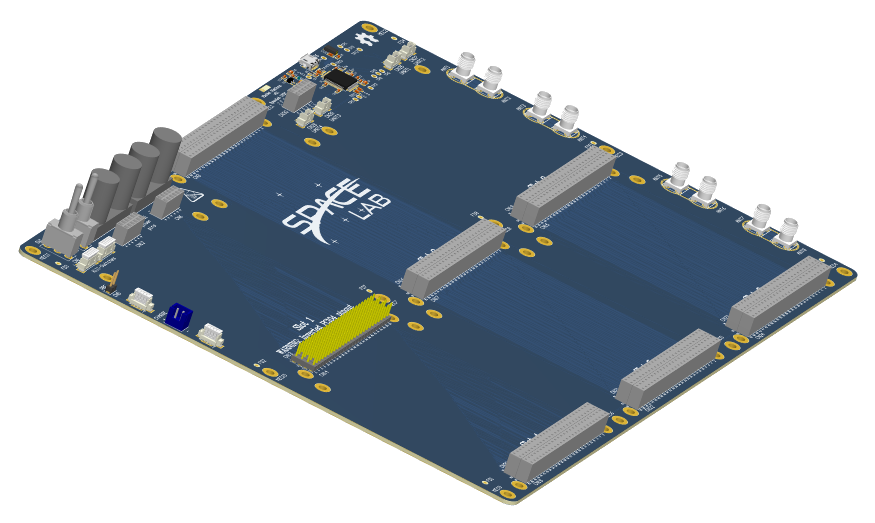
\includegraphics[width=0.75\textwidth]{figures/flatsat_perspective_image.png}
        \caption{3D view of the FlatSat PCB.}
        \label{fig:pcb-3d}
    \end{center}
\end{figure}

All the project, source and documentation files are available freely on a GitHub repository \cite{interface-board-repo} under its respective licenses.
    %
% system_overview.tex
%
% Copyright (C) 2020 by SpaceLab.
%
% Flatsat Platform Documentation
%
% This work is licensed under the Creative Commons Attribution-ShareAlike 4.0
% International License. To view a copy of this license,
% visit http://creativecommons.org/licenses/by-sa/4.0/.
%

%
% \brief System Overview chapter.
%
% \authors: Gabriel Mariano Marcelino <gabriel.marcelino@spacelab.ufsc.br> and Yan Castro de Azeredo <yan.azeredo@spacelab.ufsc.br>
%
% \institution Universidade Federal de Santa Catarina (UFSC)
%
% \version 0.1.1
%
% \date 2020/12/17
%

\chapter{System Overview} \label{ch:system-overview}

The FlatSat form factor choosen for this project is a retangular one piece design. On its current version v0.1 the platform can be purelly used hardware wise. The hardware block diagram can be seen on figure \ref{fig:block-diagram}. The PC104 slot Nº7 is supossed to be used for a extra interface, shield or another FlatSat platform.

\section{Block Diagram}

\begin{figure}[!ht]
    \begin{center}
        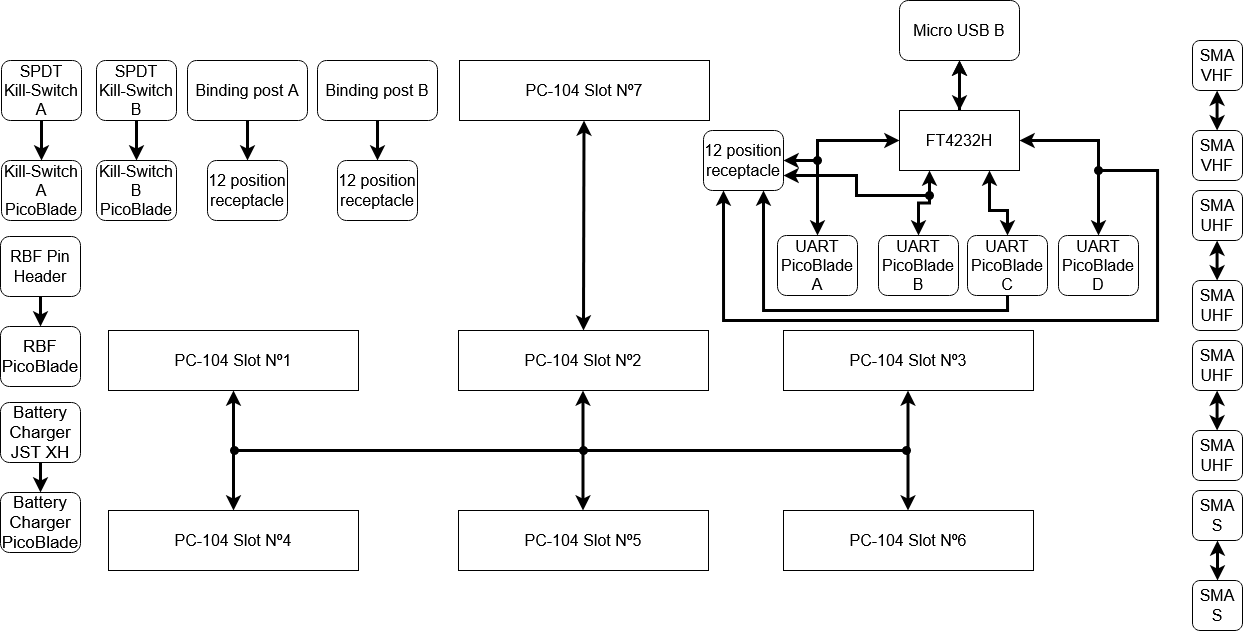
\includegraphics[width=\textwidth]{figures/flatsat_block_diagram.png}
        \caption{FlatSat hardware block diagram.}
        \label{fig:block-diagram}
    \end{center}
\end{figure}

\section{Board Dimensions}

The board is a retangular PCB with linear dimensions of 300mmx220mm. The full mechanical specs of the platform can be seen on its draftsman document available at it's GitHub repository \cite{flatsat-draftsman}.
    %
% hardware.tex
%
% Copyright (C) 2021 by SpaceLab.
%
% Flatsat Platform Documentation
%
% This work is licensed under the Creative Commons Attribution-ShareAlike 4.0
% International License. To view a copy of this license,
% visit http://creativecommons.org/licenses/by-sa/4.0/.
%

%
% \brief Hardware chapter.
%
% \author Gabriel Mariano Marcelino <gabriel.marcelino@spacelab.ufsc.br>
% \author Yan Castro de Azeredo <yan.azeredo@spacelab.ufsc.br>
%
% \institution Universidade Federal de Santa Catarina (UFSC)
%
% \version 0.2.0
%
% \date 2020/10/11
%

\chapter{Hardware} \label{ch:hardware}

This chapter describes all the FlatSat's hardware interfaces in detail. On Figures \ref{fig:pcb-top} and \ref{fig:pcb-bottom} are displayed de top and bottom PCB prints.

\begin{figure}[!ht]
    \begin{center}
        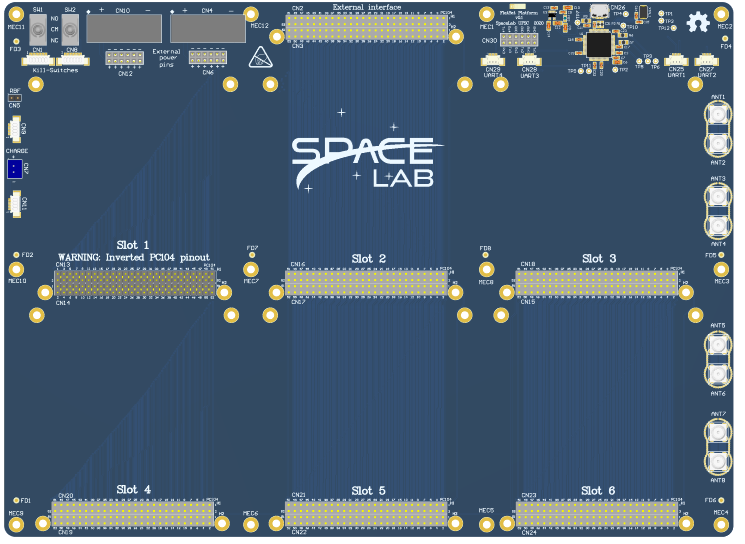
\includegraphics[width=0.8\textwidth]{figures/flatsat_top_image.png}
        \caption{FlatSat top PCB print.}
        \label{fig:pcb-top}
    \end{center}
\end{figure}

\begin{figure}[!ht]
    \begin{center}
        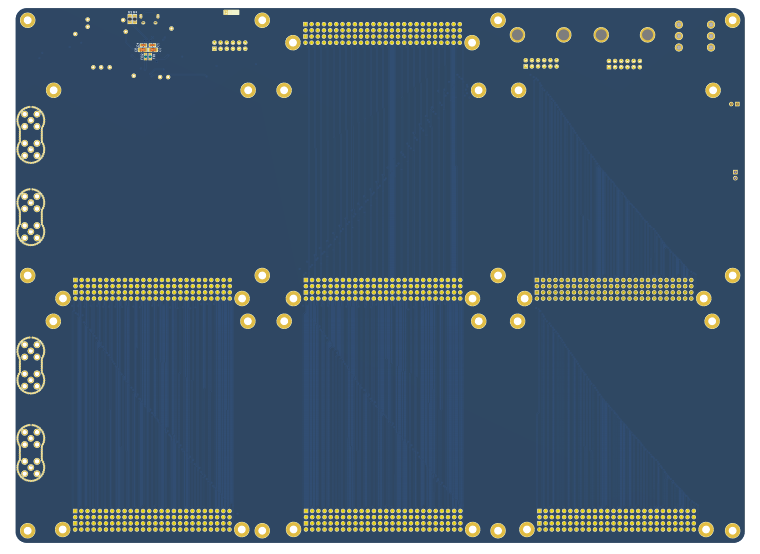
\includegraphics[width=0.8\textwidth]{figures/flatsat_bottom_image.png}
        \caption{FlatSat bottom PCB print.}
        \label{fig:pcb-bottom}
    \end{center}
\end{figure}

\section{PC-104 Interfaces}

On SpaceLab's FlatSat Platform the PC-104 interfaces are composed by two 52 pins with 2.54 mm (0.1 inch) pitch connectors. Slots N$^{\circ}$2 to N$^{\circ}$7 has two \textit{SSW-126-01-G-D} and the slot N$^{\circ}$1 uses two \textit{TSW-126-07-G-D} connectors with inverted pinout, see Figures \ref{fig:n2-n7-slots} and \ref{fig:n1-slot}. All pins are interconected to flexiblesize the positioning of the modules on the platform. All slots have grounded unlabeled mounting holes for the modules, the labeled MEC1 to MEC12 holes are for the FlatStats stability feet.

\begin{figure}[!ht]
    \begin{center}
        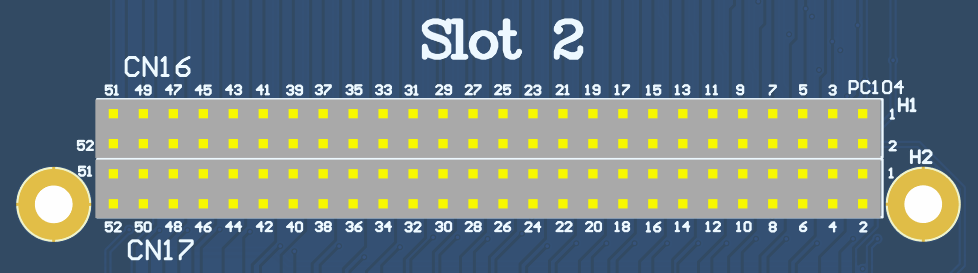
\includegraphics[width=0.75\textwidth]{figures/pc104_slots_n2_to_n7.png}
        \caption{FlatSat N$^{\circ}$2 PC-104 slot.}
        \label{fig:n2-n7-slots}
    \end{center}
\end{figure}

\begin{figure}[!ht]
    \begin{center}
        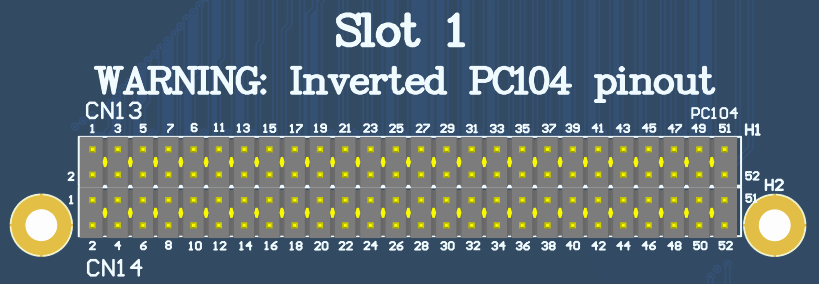
\includegraphics[width=0.75\textwidth]{figures/pc104_slot_n1.png}
        \caption{FlatSat N$^{\circ}$1 PC-104 slot.}
        \label{fig:n1-slot}
    \end{center}
\end{figure}

\section{Binding Posts and Power Receptacles}

Two sets of binding posts (\textit{4243-0}) can be mouted on the labeled CN4 and CN10 hole pads to be used for two external power supplies, see \autoref{fig:binding-posts}. The modules are powered via external jumper wires to the 12 position receptacle connectors (\textit{BCS-106-L-D-TE}) labeled CN6 and CN12. On the silkscreen the plus (+) signs are the positive power pins while the minus (-) signs are the GND pins.

\begin{figure}[!ht]
    \begin{center}
        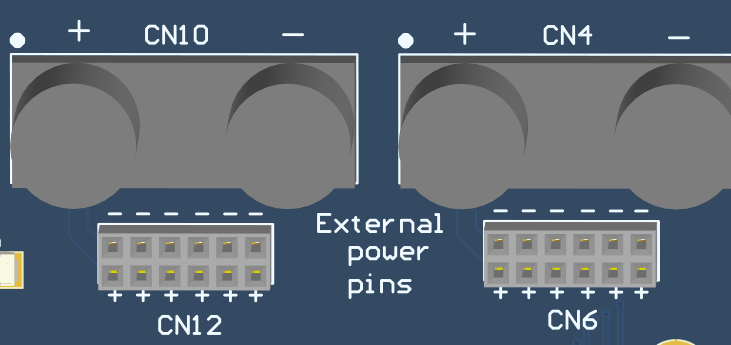
\includegraphics[width=0.75\textwidth]{figures/binding_posts.png}
        \caption{FlatSat binding posts and power receptables.}
        \label{fig:binding-posts}
    \end{center}
\end{figure}

\section{Charge Header}

On the board there is a JST XH 2 position header (\textit{B2B-XH-A-M(LF)(SN)}) for charging batteries, it can be seen in \autoref{fig:charge-connectors}. The component can suport up to 3000 mA of current, but it is advised to be used with less than 1500 mA. The 4 pin PicoBlade is to be connected to the EPS\nomenclature{\textbf{EPS}}{\textit{Electric Power System.}} module to make the interconnection for the JST header. The charge header also provides a detent lock for fastening and avoid a mistankenly reverse connection.

\begin{figure}[!ht]
    \begin{center}
        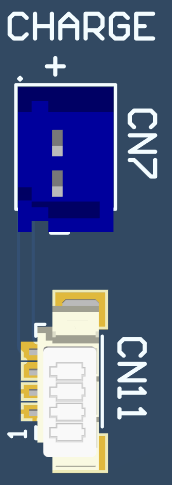
\includegraphics[width=0.15\textwidth]{figures/charge_connectors.png}
        \caption{FlatSat charge connectors.}
        \label{fig:charge-connectors}
    \end{center}
\end{figure}

\section{RBF Pin Header}

The platform has a RBF pin header that can seen \autoref{fig:rbf-connectors}. The interconnection between the header and the EPS module is done by a 4 pin PicoBlade.

\begin{figure}[!ht]
    \begin{center}
        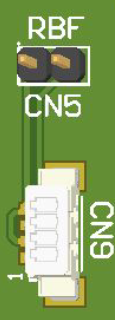
\includegraphics[width=0.15\textwidth]{figures/rbf_connectors.png}
        \caption{FlatSat RBF connectors.}
        \label{fig:rbf-connectors}
    \end{center}
\end{figure}

\section {SPDT Kill-Switches}

The kill-switches uses SPDT switches (\textit{100SP1T1B4M2QE}) for powering off the EPS module, see \autoref{fig:kill-switches-connectors}. The power off states are seen on \autoref{fig:kill-switches-states}, they are also present on the hardware schematics. The SPDTs are interconnected to the EPS module via two 6 pin PicoBlade connectors labeled CN1 and CN8.

\begin{figure}[!ht]
    \begin{center}
        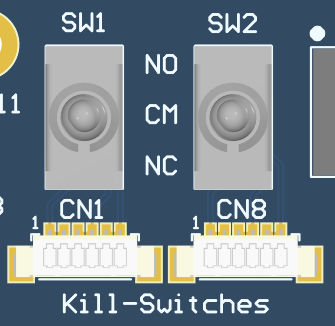
\includegraphics[width=0.5\textwidth]{figures/kill_switches_connectors.png}
        \caption{FlatSat kill-switches connectors.}
        \label{fig:kill-switches-connectors}
    \end{center}
\end{figure}

\begin{figure}[!ht]
    \begin{center}
        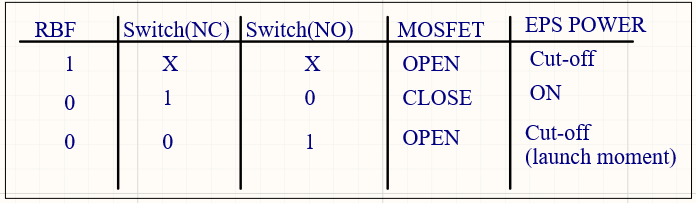
\includegraphics[width=0.75\textwidth]{figures/kill_switches_states.png}
        \caption{FlatSat kill-switches states.}
        \label{fig:kill-switches-states}
    \end{center}
\end{figure}

\section{Antenna Interfaces}

\subsection{SMA connectors}

On the PCB there are SMA connectors (\textit{132134-15}) labeled ANT1 to ANT8 for connecting VHF\nomenclature{\textbf{VHF}}{\textit{Very High Frequency.}}, UHF\nomenclature{\textbf{UHF}}{\textit{Ultra High Frequency.}} and S-Band antennas, see \autoref{fig:antennas-smas}. The receiver (RX) antenna is to be connected to one of the SMA, while the transmitter (TX) goes to the other connector and to the CubeSat module. The impedance control (see \autoref{fig:rf-track-width-calc}) and power dissipation (see \autoref{fig:rf-track-width-power-calc}) where approximately calculated for all 3 bands. As the FlatSat platform is to be used in light testing the aproximations where considered acceptable for the project.

\begin{figure}[!ht]
    \begin{center}
        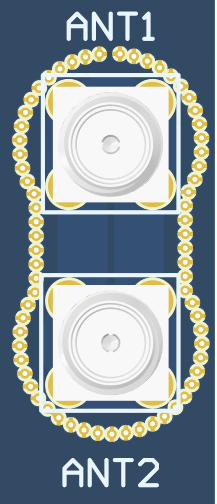
\includegraphics[width=0.15\textwidth]{figures/antennas_smas.png}
        \caption{FlatSat SMA connectors.}
        \label{fig:antennas-smas}
    \end{center}
\end{figure}

\subsection{Impedance Control of the RF Tracks}

\begin{figure}[!ht]
    \begin{center}
        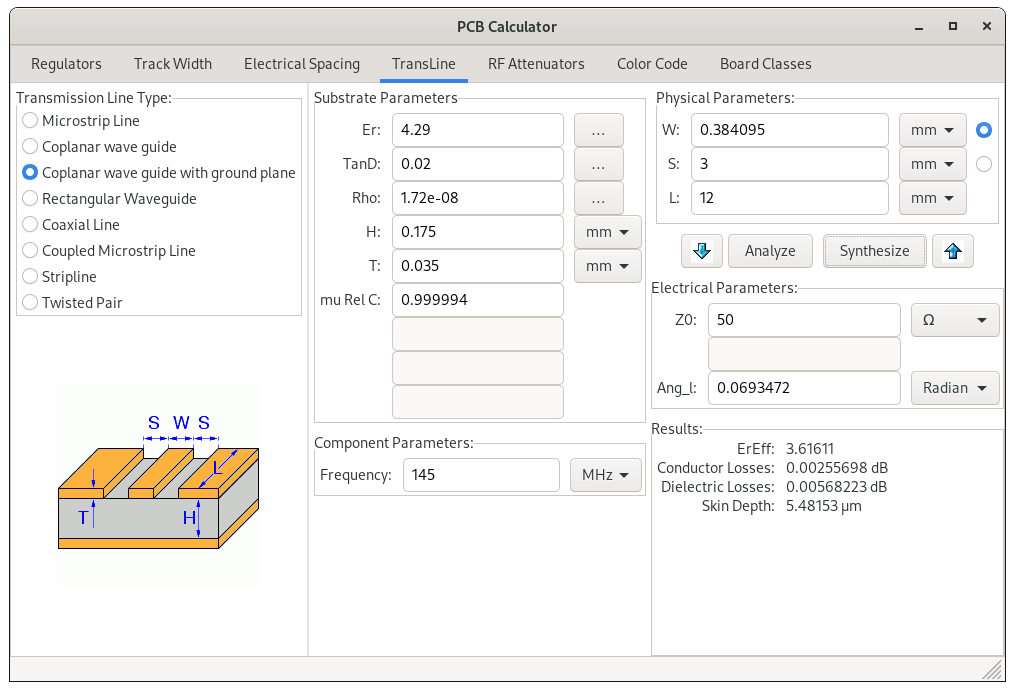
\includegraphics[width=\textwidth]{figures/rf-track-width.png}
        \caption{Calculation of the width of the RF tracks.}
        \label{fig:rf-track-width-calc}
    \end{center}
\end{figure}

\begin{figure}[!ht]
    \begin{center}
        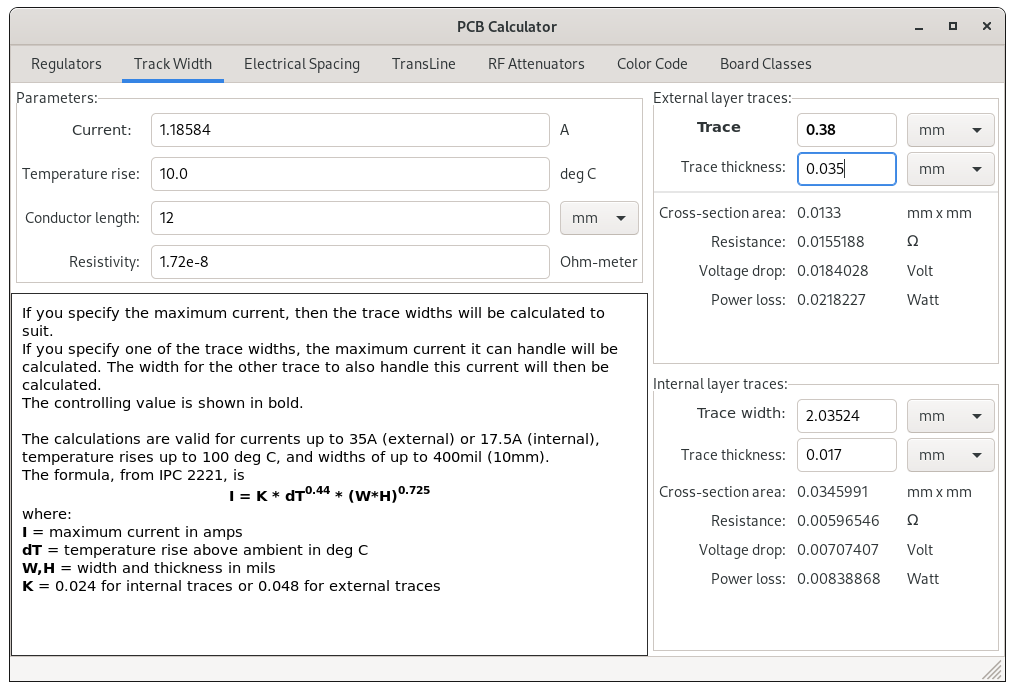
\includegraphics[width=\textwidth]{figures/rf-track-width-power.png}
        \caption{Power dissipation of the RF tracks.}
        \label{fig:rf-track-width-power-calc}
    \end{center}
\end{figure}

\section{UART to USB Converter}

There is a UART to USB converter circuit built-in the FlatSat platform for debbuging pourposes for four independent modules, it can be seen on \autoref{fig:ft4232h-circuit}. The subcircuit is self powered from a USB cable connecting a computer to a micro USB type B port (\textit{10118194-0001LF}). The USB Bridge converter IC\nomenclature{\textbf{IC}}{\textit{Integrated Circuit.}} is the \textit{FT4232HL-REEL} from FTDI. PicoBlade connectors are used for connecting the IC to the modules, see Figures \ref{fig:uart-picoblades-1} and \ref{fig:uart-picoblades-2}. It is also possible to use jumper wires connecting the 12 Position receptacle connector (\textit{BCS-106-L-D-TE}) labeled CN30 to the modules if PicoBlades are not used.

\begin{figure}[!ht]
    \begin{center}
        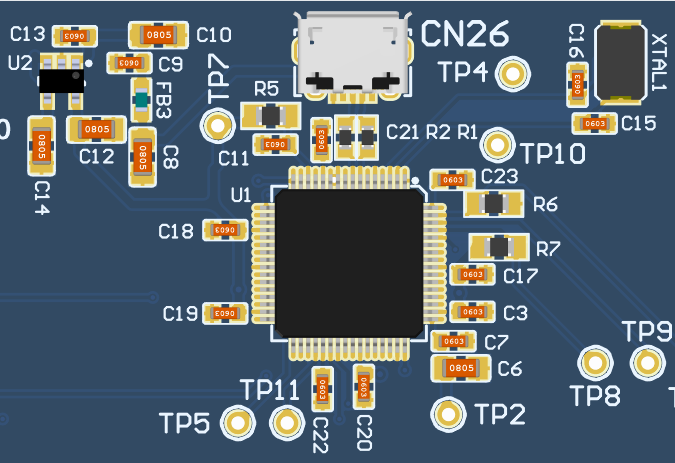
\includegraphics[width=0.75\textwidth]{figures/ft4232h_circuit.png}
        \caption{Top view of the UART to USB converter circuit.}
        \label{fig:ft4232h-circuit}
    \end{center}
\end{figure}

\begin{figure}[!ht]
    \begin{center}
        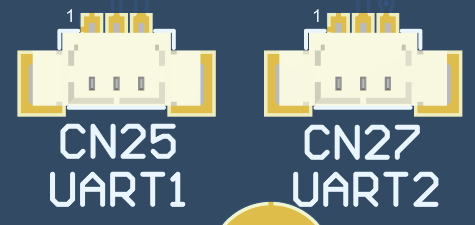
\includegraphics[width=0.5\textwidth]{figures/picoblade_uarts_n1_and_n2}
        \caption{UART PicoBlade N$^{\circ}$1 and N$^{\circ}$2 connectors.}
        \label{fig:uart-picoblades-1}
        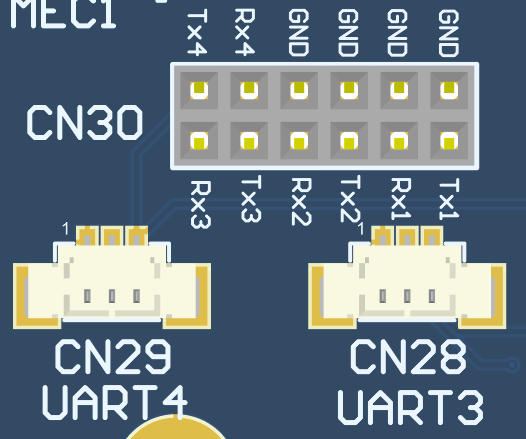
\includegraphics[width=0.5\textwidth]{figures/picoblade_uarts_n3_and_n4_and_receptable.png}
        \caption{UART PicoBlade N$^{\circ}$3 and N$^{\circ}$4 connectors and receptable.}
        \label{fig:uart-picoblades-2}
    \end{center}
\end{figure}

\section{Test Points}

The FlatSat has test points for the UART to USB converter circuit. The \autoref{tab:testpoints} displays their labels and description.

\begin{table}[!h]
    \centering
    \begin{tabular}{cllll}
        \toprule[1.5pt]
        \textit{Label} & \textit{Description} \\
        \midrule
        TP1                & (VPLL) 3V3 FT4232H power input. \\
        TP2                & (VREGOUT) 1V8 FT4232H internal power output. \\
        TP3                & (VPHY) 3V3 FT4232H power input. \\
        TP4                & (REF) Current reference for FT4232H. \\
        TP5                & (RESET\#) Reset input for FT4232H. \\
        TP6                & (EECS) EEPROM chip select - pulled down by 10k resistor. \\
        TP7                & (VCCIO) I/O interface 3V3 power supply input. \\
        TP8                & (EEDATA) EEPROM data I/O - pulled up by 10k resistor. \\
        TP9                & (EECLK) Clock signal to EEPROM - not used. \\
        TP10               & (PWREN\#) Active low power-enable output. \\
        TP11               & (SUSPEND\#) Active low when USB is in suspend mode. \\
        TP12               & (GND) 0V ground input for FT4232H.\\
        \bottomrule[1.5pt]
    \end{tabular}
    \caption{FlatSat test points.}
    \label{tab:testpoints}
\end{table}

    %
% assembly.tex
%
% Copyright (C) 2021 by SpaceLab.
%
% Flatsat Platform Documentation
%
% This work is licensed under the Creative Commons Attribution-ShareAlike 4.0
% International License. To view a copy of this license,
% visit http://creativecommons.org/licenses/by-sa/4.0/.
%

%
% \brief Board Assembly chapter.
%
% \author Gabriel Mariano Marcelino <gabriel.marcelino@spacelab.ufsc.br>
% \author Yan Castro de Azeredo <yan.azeredo@spacelab.ufsc.br>
%
% \institution Universidade Federal de Santa Catarina (UFSC)
%
% \version 0.1.0
%
% \date 2020/24/12
%

\chapter{Board Assembly}

The hardware project has the Bill of Material (BOM) avalaible at its GitHub repository in excel spreeadsheets format. The PCB can be assembled by a Pick-and-place machine using the .txt file found on the hardware/fabrication folder if desired, fiducials labeled FD\# are placed to make this possible.

\section{FlatSat Stabillity Feet}

On the PCB there are labeled MEC1 to MEC12 mouting holes on the edges and in the middle of the board to be used for stabillity feet when the board is placed on top of a test bench.

\section{DNP Components}

There is only one Do Not Place (DNP) component present in the USB to UART circuit, it is the labeled R4 pad with 0805 size (2012 metric) available for soldering the micro USB type B chassi to GND for Electromagnetic compatibility (EMC) see \autoref{fig:R4-pad}. This can be done soldering a zero-Ohm resistor for a DC path or capacitor for a high-frequency path between shield and signal ground, see section 2.2.2 of the document \cite{ftdi-usb-hardware-guidelines} for more details.

\begin{figure}[!ht]
    \begin{center}
        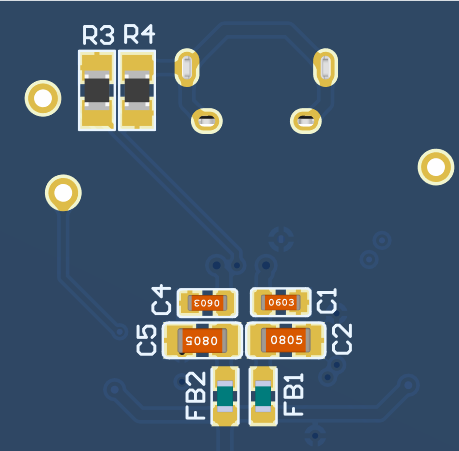
\includegraphics[width=0.5\textwidth]{figures/ft4232h_circuit_bottom.png}
        \caption{Bottom view of the UART to USB converter circuit.}
        \label{fig:R4-pad}
    \end{center}
\end{figure}

\section{Modules Mounting}

The PC-104 slots N$^{\circ}$2 to N$^{\circ}$7 are compatible for CubeSat PCB modules that are stacked in middle or the first on top. The slot N$^{\circ}$1 can only be used for the last module on this stack because of the inverted pinout. For the case of the SpaceLab's CubeSat stackup of the core modules, the last module of the stack is the EPS. For this case the EPS needs to be mounted up-side-down on slot N$^{\circ}$1 as can be seen on \autoref{fig:eps2-mouting}. For other modules any other PC-104 slots can be used, the OBDH is showed mouted on \autoref{fig:obdh2-mouting}.

\begin{figure}[!ht]
    \begin{center}
        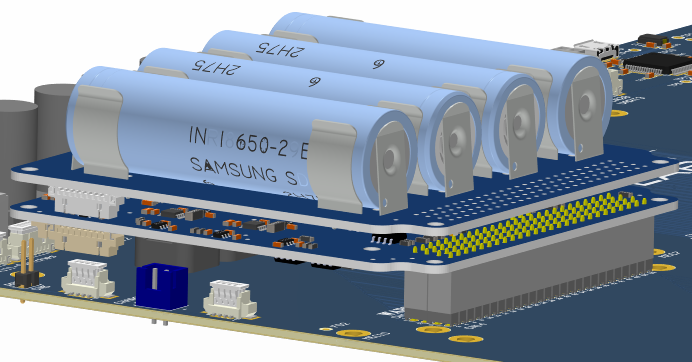
\includegraphics[width=0.8\textwidth]{figures/eps2_mouting.png}
        \caption{EPS mounted on N$^{\circ}$1 slot on a EDA tool.}
        \label{fig:eps2-mouting}
    \end{center}
\end{figure}

\begin{figure}[!ht]
    \begin{center}
        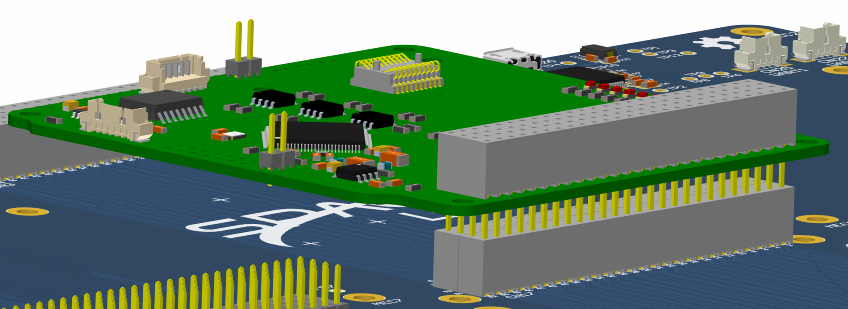
\includegraphics[width=0.8\textwidth]{figures/obdh2_mouting.png}
        \caption{OBDH mounted on N$^{\circ}$2 slot on a EDA tool.}
        \label{fig:obdh2-mouting}
    \end{center}
\end{figure}

\section{Antennas Connection}

Since the SMA connectors present on the board are on the right far side, modules placed in the opposite side may not be in reach for the connection. Because of this reason is recommended to use slots N$^{\circ}$1 and N$^{\circ}$4 for non antenna dependents PCBs.

    %
% intructions.tex
%
% Copyright (C) 2021 by SpaceLab.
%
% Flatsat Platform Documentation
%
% This work is licensed under the Creative Commons Attribution-ShareAlike 4.0
% International License. To view a copy of this license,
% visit http://creativecommons.org/licenses/by-sa/4.0/.
%

%
% \brief Usage Instructions chapter.
%
% \author Yan Castro de Azeredo <yan.azeredo@spacelab.ufsc.br>
%
% \institution Universidade Federal de Santa Catarina (UFSC)
%
% \version 0.2.0
%
% \date 2020/04/01
%

\chapter{Usage Instructions} \label{ch:instructions}

\section{Charging Batteries Through Connector}

To charge the batteries it will be needed a cable compatible with the JST XH header. The compatible housing is a XHP-2 receptacle, the jumper lead socket to socket to be used can be \textit{ASXHSXH22K305}, or any other with AWG\nomenclature{\textbf{AWG}}{\textit{American Wire Gauge.}} \#30 to \#22. The only constraint is that the current cannot excel 2000 mA, because the PicoBlades connectors used to interconnect the JST header to the EPS only supports 1000 mA per pin. For safe usage it is recommended to use the header with a maximum of 1500 mA charge current.

\section{Debugging Though USB}

Connecting a type A to micro type B USB cable to a PC\nomenclature{\textbf{PC}}{\textit{Personal Computer.}} and the USB port present on the FlatSat, the four USB to UART channels should be ready to be used. Note that the computer will recognize the port as four different devices. The FT4232H IC present on the platform  doesn't have an EEPROM\nomenclature{\textbf{EEPROM}}{\textit{Electrically-Erasable Programmable Read-Only Memory.}}, so it will be already configured to operate as default serial ports. The FT4232H will have the built-in default VID (0403) and PID (6011).

\section{Debugging Though PC-104}

Since all PC-104 interfaces are interconnected any slot can be used for probing and debbuging. Intentionally the slot N$^{\circ}$7 or also labeled ``external interface'' on the PCB was meant to be used for testing all pins. A new board or another FlatSat platform can be connected to this interface if the pinout of the specific project is compatible. The GOLDS-UFSC pinout is avalaible at its github repository \cite{golds-ufsc}.

    %
% references.tex
%
% Copyright (C) 2020 by SpaceLab.
%
% Flatsat Platform Documentation
%
% This work is licensed under the Creative Commons Attribution-ShareAlike 4.0
% International License. To view a copy of this license,
% visit http://creativecommons.org/licenses/by-sa/4.0/.
%

%
% \brief References chapter.
%
% \author Gabriel Mariano Marcelino <gabriel.mm8@gmail.com>
%
% \institution Universidade Federal de Santa Catarina (UFSC)
%
% \version 0.1.0
%
% \date 2020/07/16
%

\bibliography{references/test,references/obdh2}

\addcontentsline{toc}{chapter}{References}


\end{document}
